%%% Credit: user:cfr - tex.stackexchange.com
\documentclass{article}
\usepackage{silence}
\WarningFilter{latex}{Writing}
\usepackage{standalone}
\usepackage{tikz}
\usetikzlibrary{
  matrix,
  calc,
  positioning,
  arrows,
  intersections,
  math,
  circuits.ee.IEC,
  external}
\usepackage{pgfplots}
  \usepgfplotslibrary{external}
  \pgfplotsset{compat=1.18}
\usepackage{ifthen}
\usepackage{amssymb}
\usepackage{currfile}
\usepackage{etoolbox}

\tikzexternalize[prefix=./]
\tikzsetfigurename{figure-}
\newcommand*\setmyname{%
  \expandafter\tikzsetfigurename\expandafter{\currfilebase-}%
}
\makeatletter
\apptocmd{\sa@document}{\setmyname}{\typeout{Append to document: OK!}}{\typeout{Append to document: Oh, no!}}
\makeatother

\begin{filecontents*}[overwrite]{plot.tex}
\documentclass[tikz]{standalone}
\usepackage{pgfplots}
  \usetikzlibrary{positioning}
  \usepgfplotslibrary{external}
  \pgfplotsset{
    % width=10cm,
    compat=1.18
  }
\begin{document}

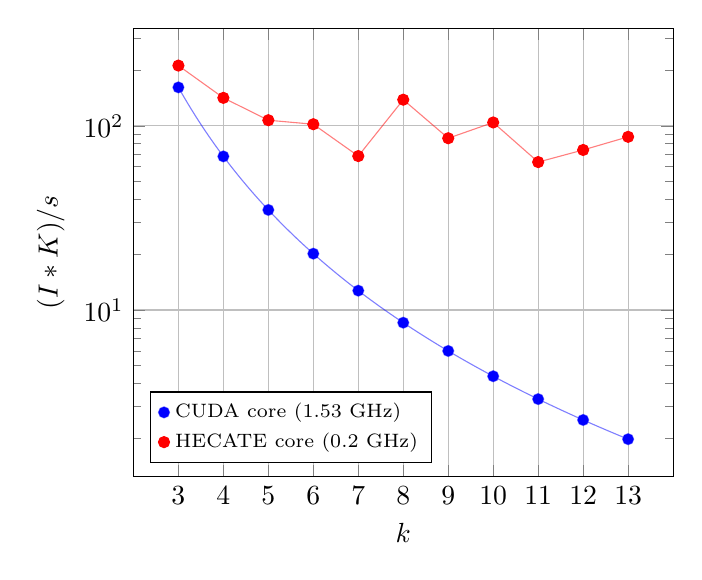
\begin{tikzpicture}
  \begin{semilogyaxis}[
    domain=3:13,
    xtick={3,...,13},
    % y domain=3:11, 
    grid=major,
    xlabel=$k$,
    ylabel=$(I*K)/s$,
    legend style={font=\scriptsize},
    legend cell align=left,
    legend pos=south west,
    % colormap={bw},
  ]
    \addplot[
      scatter src=none,
      samples=11,
      only marks,
      color=blue,
      draw opacity=0.5,
    ]{
      (1/((128*171*16)*x^3))*1530000000
    };
    \addplot[
      samples=100,
      color=blue,
      draw opacity=0.5,
    ]{
      (1/((128*171*16)*x^3))*1530000000
    };
    \addplot[
      scatter src=none,
      samples=11,
      color=red,
      only marks
    ]{
      (2/(
        (ceil(128/x) * ceil(171/x) * ceil(16/x))
        *(pow(2,ceil(log2((2*x-1)^3))))
      ))*200000000
    };
    \addplot[
      samples=11,
      draw opacity=0.5,
      color=red,
    ]{
      (2/(
        (ceil(128/x) * ceil(171/x) * ceil(16/x))
        *(pow(2,ceil(log2((2*x-1)^3))))
      ))*200000000
    };
    % \addplot[
    %   samples=100,
    %   draw opacity=0.5,
    %   color=green,
    % ]{
    %   (2/(((128*171*16)/(x^3))*((2*x-1)^3)))*200000000
    % };
  \legend{CUDA core (1.53 GHz),,HECATE core (0.2 GHz)}
  \end{semilogyaxis}
\end{tikzpicture}

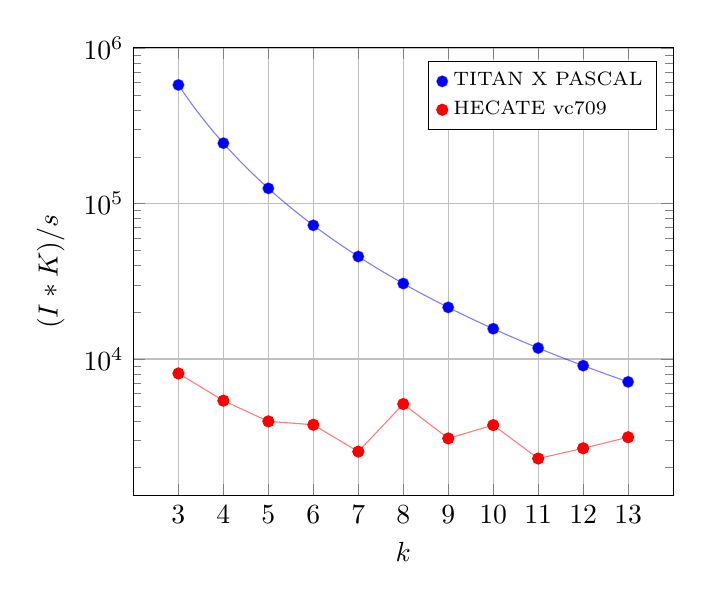
\begin{tikzpicture}
  \begin{semilogyaxis}[
    domain=3:13,
    xtick={3,...,13},
    % y domain=3:11, 
    grid=major,
    xlabel=$k$,
    ylabel=$(I*K)/s$,
    legend style={font=\scriptsize},
    legend cell align=left,
    legend pos=north east,
    % colormap={bw},
  ]
    \addplot[
      scatter src=none,
      samples=11,
      only marks,
      color=blue,
      draw opacity=0.5,
    ]{
      (3584/((128*171*16)*x^3))*1530000000
    };
    \addplot[
      samples=100,
      color=blue,
      draw opacity=0.5,
    ]{
      (3584/((128*171*16)*x^3))*1530000000
    };
    \addplot[
      scatter src=none,
      samples=11,
      color=red,
      only marks
    ]{
      ((ceil(433200/(10646+(112*ceil(log2((2*x-1)^3)))))*2)/(
        (ceil(128/x) * ceil(171/x) * ceil(16/x))
        *(pow(2,ceil(log2((2*x-1)^3))))
      ))*200000000
    };
    \addplot[
      samples=11,
      draw opacity=0.5,
      color=red,
    ]{
      ((ceil(433200/(10646+(112*ceil(log2((2*x-1)^3)))))*2)/(
        (ceil(128/x) * ceil(171/x) * ceil(16/x))
        *(pow(2,ceil(log2((2*x-1)^3))))
      ))*200000000
    };
    % \addplot[
    %   samples=100,
    %   draw opacity=0.5,
    %   color=green,
    % ]{
    %   (2/(((128*171*16)/(x^3))*((2*x-1)^3)))*200000000
    % };
  \legend{TITAN X PASCAL,,HECATE vc709}
  \end{semilogyaxis}
\end{tikzpicture}

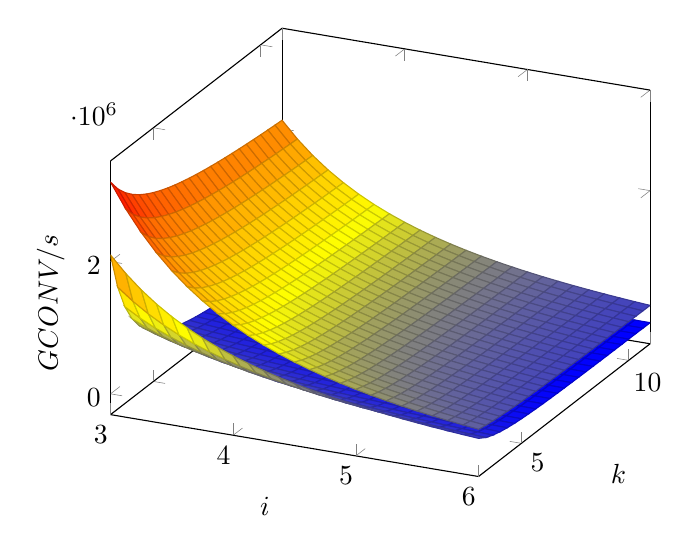
\begin{tikzpicture}
  \begin{axis}[
    domain=3:6,
    y domain=3:11, 
    % samples=100,
    % grid=major,
    restrict z to domain=0:10^9,
    xlabel=$i$,
    ylabel=$k$,
    zlabel=$GCONV/s$,
    legend pos=north west
  ]
    \addplot3[
      surf
    ]{
      (1/(x^3*y^3))*1530000000
    };
    \addplot3[
      surf
    ]{
      (2/(((x^3)/(y^3))*((2*y-1)^3)))*200000000
    };
  \end{axis}
\end{tikzpicture}

\end{document}
\end{filecontents*}

\begin{filecontents*}[overwrite]{matrix.tex}
\documentclass[tikz]{standalone}
\begin{document}
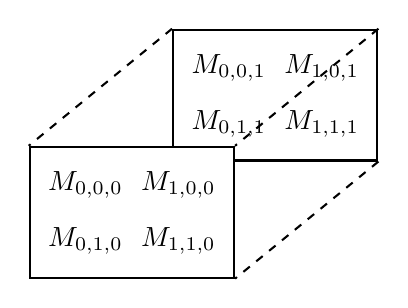
\begin{tikzpicture}[
  >=stealth,
  line width=0.75pt,
  every node/.style={anchor=north east,fill=white,minimum width=1.1cm,minimum height=7mm},
  ampersand replacement=\&
]%
  \matrix (mA) [draw,matrix of math nodes]
  {
    M_{0,0,1} \& M_{1,0,1} \\
    M_{0,1,1} \& M_{1,1,1} \\
  };

  \matrix (mB) [draw,matrix of math nodes] at ($(mA.south west)+(0.8,0.2)$)
  {
    M_{0,0,0} \& M_{1,0,0} \\
    M_{0,1,0} \& M_{1,1,0} \\
  };

  \draw[dashed](mA.north east)--(mB.north east);
  \draw[dashed](mA.north west)--(mB.north west);
  \draw[dashed](mA.south east)--(mB.south east);
\end{tikzpicture}
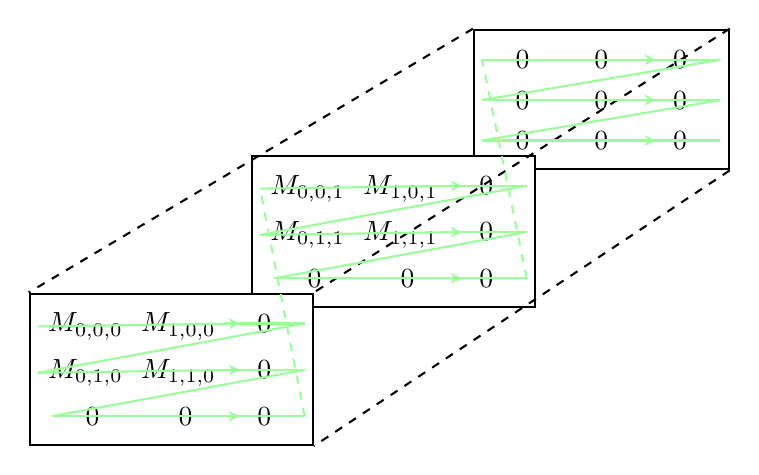
\begin{tikzpicture}[
  >=stealth,
  line width=0.75pt,
  every node/.style={anchor=north east,fill=white,minimum width=1.0cm,minimum height=5mm},
  ampersand replacement=\&
]%
  \matrix (mA) [draw,matrix of math nodes]
  {
    |(mA1)| 0 \& 0 \& |(mA2)| 0 \\
    |(mA3)| 0 \& 0 \& |(mA4)| 0 \\
    |(mA5)| 0 \& 0 \& |(mA6)| 0 \\
  };

  \matrix (mB) [draw,matrix of math nodes] at ($(mA.south west)+(0.8,0.2)$)
  {
    |(mB1)| M_{0,0,1} \& M_{1,0,1} \& |(mB2)| 0 \\
    |(mB3)| M_{0,1,1} \& M_{1,1,1} \& |(mB4)| 0 \\
    |(mB5)| 0         \& 0         \& |(mB6)| 0 \\
  };

  \matrix (mC) [draw,matrix of math nodes] at ($(mB.south west)+(0.8,0.2)$)
  {
    |(mC1)| M_{0,0,0} \& M_{1,0,0} \& |(mC2)| 0 \\
    |(mC3)| M_{0,1,0} \& M_{1,1,0} \& |(mC4)| 0 \\
    |(mC5)| 0         \& 0         \& |(mC6)| 0 \\
  };

  \draw[dashed](mA.north east)--(mC.north east);
  \draw[dashed](mA.north west)--(mC.north west);
  \draw[dashed](mA.south east)--(mC.south east);

  \draw[->,color=green!40]     (mC1.west) -- ($(mC2.west)+(0.2,0)$);
  \draw[color=green!40]        (mC2.west) -- (mC2.east);
  \draw[color=green!40]        (mC2.east) -- (mC3.west);
  \draw[->,color=green!40]     (mC3.west) -- ($(mC4.west)+(0.2,0)$);
  \draw[color=green!40]        (mC4.west) -- (mC4.east);
  \draw[color=green!40]        (mC4.east) -- (mC5.west);
  \draw[->,color=green!40]     (mC5.west) -- ($(mC6.west)+(0.2,0)$);
  \draw[color=green!40]        (mC6.west) -- (mC6.east);
  \draw[dashed,color=green!40] (mC6.east) -- (mB1.west);

  \draw[->,color=green!40]     (mB1.west) -- ($(mB2.west)+(0.2,0)$);
  \draw[color=green!40]        (mB2.west) -- (mB2.east);
  \draw[color=green!40]        (mB2.east) -- (mB3.west);
  \draw[->,color=green!40]     (mB3.west) -- ($(mB4.west)+(0.2,0)$);
  \draw[color=green!40]        (mB4.west) -- (mB4.east);
  \draw[color=green!40]        (mB4.east) -- (mB5.west);
  \draw[->,color=green!40]     (mB5.west) -- ($(mB6.west)+(0.2,0)$);
  \draw[color=green!40]        (mB6.west) -- (mB6.east);
  \draw[dashed,color=green!40] (mB6.east) -- (mA1.west);

  \draw[->,color=green!40]     (mA1.west) -- ($(mA2.west)+(0.2,0)$);
  \draw[color=green!40]        (mA2.west) -- (mA2.east);
  \draw[color=green!40]        (mA2.east) -- (mA3.west);
  \draw[->,color=green!40]     (mA3.west) -- ($(mA4.west)+(0.2,0)$);
  \draw[color=green!40]        (mA4.west) -- (mA4.east);
  \draw[color=green!40]        (mA4.east) -- (mA5.west);
  \draw[->,color=green!40]     (mA5.west) -- ($(mA6.west)+(0.2,0)$);
  \draw[color=green!40]        (mA6.west) -- (mA6.east);

\end{tikzpicture}
\end{document}
\end{filecontents*}

\begin{filecontents*}[overwrite]{unit_circle.tex}
\documentclass[tikz]{standalone}
\begin{document}
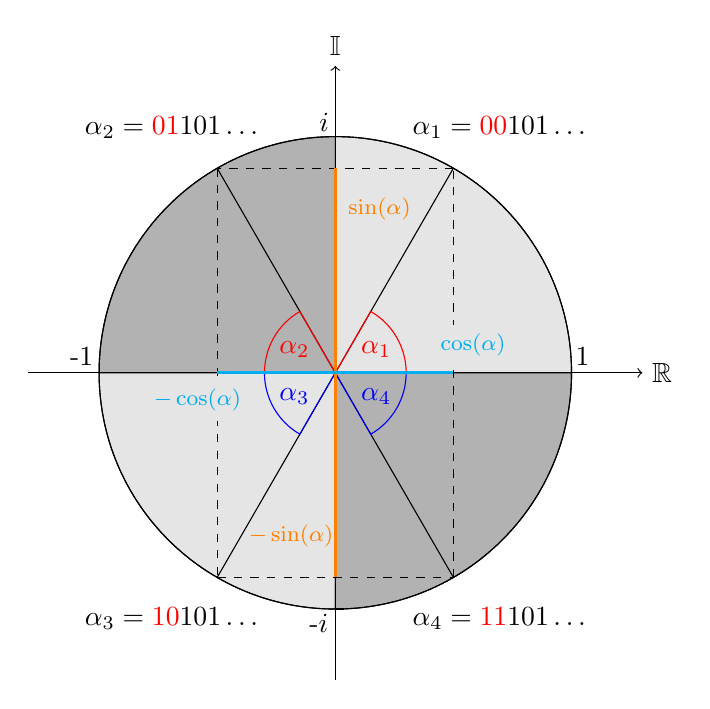
\begin{tikzpicture}[
  scale=3
]%
  % Quadrants
  \filldraw[fill=gray!20,draw]
    (0,0) -- (1 cm,0pt) arc [start angle=0, end angle=90, radius=1cm] -- cycle;
  \filldraw[fill=gray!60,draw]
    (0,0) -- (0pt,1 cm) arc [start angle=90, end angle=180, radius=1cm] -- cycle;
  \filldraw[fill=gray!20,draw]
    (0,0) -- (-1 cm,0pt) arc [start angle=180, end angle=270, radius=1cm] -- cycle;
  \filldraw[fill=gray!60,draw]
    (0,0) -- (0pt,- 1cm) arc [start angle=270, end angle=360, radius=1cm] -- cycle;

  % Unit circle and lines
  \path [name path=unit circle,draw] (0,0) circle [radius=1cm];
  \path [name path=q1 line,draw] (0,0) -- (60:1.0cm);
  \path [name path=q2 line,draw] (0,0) -- (120:1.0cm);
  \path [name path=q3 line,draw] (0,0) -- (240:1.0cm);
  \path [name path=q4 line,draw] (0,0) -- (300:1.0cm);

  % Grid and coordinate plane
  % \draw[step=.5cm,gray,very thin] (-1.2,-1.2) grid (1.2,1.2);
  \draw[->] (-1.3,0) -- (1.3,0) coordinate (x axis)node[right]{$\mathbb{R}$};
  \draw[->] (0,-1.3) -- (0,1.3) coordinate (y axis)node[above]{$\mathbb{I}$};
  \draw (1 cm,1pt) -- (1 cm,0pt) node[anchor=east,xshift=10pt,yshift=6pt] {$1$};
  \draw (-1 cm,1pt) -- (-1 cm,0pt) node[anchor=west,xshift=-14pt,yshift=6pt] {-$1$};
  \draw (1pt,1 cm) -- (0pt, 1 cm) node[anchor=north,xshift=-4pt,yshift=12pt] {$i$};
  \draw (1pt,-1 cm) -- (0pt, -1 cm) node[anchor=south,xshift=-6pt,yshift=-12pt] {-$i$};

  % Angles
  \path[draw=red]
    (0,0) -- (3mm,0mm) arc [start angle=0, end angle=60, radius=3mm] -- cycle;
  \node[red] at (30:2mm) {$\alpha_1$};

  \path[draw=red]
    (0,0) -- (-3mm,0mm) arc [start angle=180, end angle=120, radius=3mm] -- cycle;
  \node[red] at (150:2mm) {$\alpha_2$};

  \path[draw=blue]
    (0,0) -- (-3mm,0mm) arc [start angle=180, end angle=240, radius=3mm] -- cycle;
  \node[blue] at (210:2mm) {$\alpha_3$};

  \path[draw=blue]
    (0,0) -- (3mm,0mm) arc [start angle=0, end angle=-60, radius=3mm] -- cycle;
  \node[blue] at (-30:2mm) {$\alpha_4$};

  % Reflections
  \path [name intersections={of=unit circle and q1 line, by=q1inter}] (0,0);
  \path [name intersections={of=unit circle and q2 line, by=q2inter}] (0,0);
  \path [name intersections={of=unit circle and q3 line, by=q3inter}] (0,0);
  \path [name intersections={of=unit circle and q4 line, by=q4inter}] (0,0);

  \draw [dashed] (q1inter) -- (q2inter);
  \draw [dashed] (q2inter) -- (q3inter);
  \draw [dashed] (q3inter) -- (q4inter);
  \draw [dashed] (q4inter) -- (q1inter);

  % Sines and cosines
  \draw[very thick,orange]
    (0,0) -- node[above,xshift=16pt,yshift=0.5cm] {\footnotesize$\sin(\alpha)$} (y axis |- 60:1cm);
  \draw[very thick,orange]
    (0:0) -- node[below,xshift=-16pt,yshift=-0.5cm] {\footnotesize$-\sin(\alpha)$} (y axis |- 240:1cm);
  \draw[very thick,cyan]
    (0,0) -- node[above,xshift=1cm,yshift=2pt,fill=gray!20] {\footnotesize$\cos(\alpha)$} (60:1cm |- x axis);
  \draw[very thick,cyan]
    (0,0) -- node[below,xshift=-1cm,yshift=-2pt,fill=gray!20] {\footnotesize$-\cos(\alpha)$} (120:1cm |- x axis);

  % Angle descriptions
  \node[xshift=8pt] at (60:1.2 cm) {$\alpha_1 = \textcolor{red}{00}101\ldots$};
  \node[xshift=-8pt] at (120:1.2 cm) {$\alpha_2 = \textcolor{red}{01}101\ldots$};
  \node[xshift=-8pt] at (240:1.2 cm) {$\alpha_3 = \textcolor{red}{10}101\ldots$};
  \node[xshift=8pt] at (300:1.2 cm) {$\alpha_4 = \textcolor{red}{11}101\ldots$};

  % Rotated version
  % \node[rotate=-30,xshift=8pt] at (60:1.2 cm) {$\alpha_1 = \textcolor{red}{00}101\ldots$};
  % \node[rotate=30,xshift=-8pt] at (120:1.2 cm) {$\alpha_2 = \textcolor{red}{01}101\ldots$};
  % \node[rotate=-30,xshift=-8pt] at (240:1.2 cm) {$\alpha_3 = \textcolor{red}{10}101\ldots$};
  % \node[rotate=30,xshift=8pt] at (300:1.2 cm) {$\alpha_4 = \textcolor{red}{11}101\ldots$};
\end{tikzpicture}
\end{document}
\end{filecontents*}

\begin{filecontents*}[overwrite]{fft.tex}
\documentclass[tikz]{standalone}
\begin{document}
\pgfkeys{/pgf/number format/.cd,fixed,precision=2}
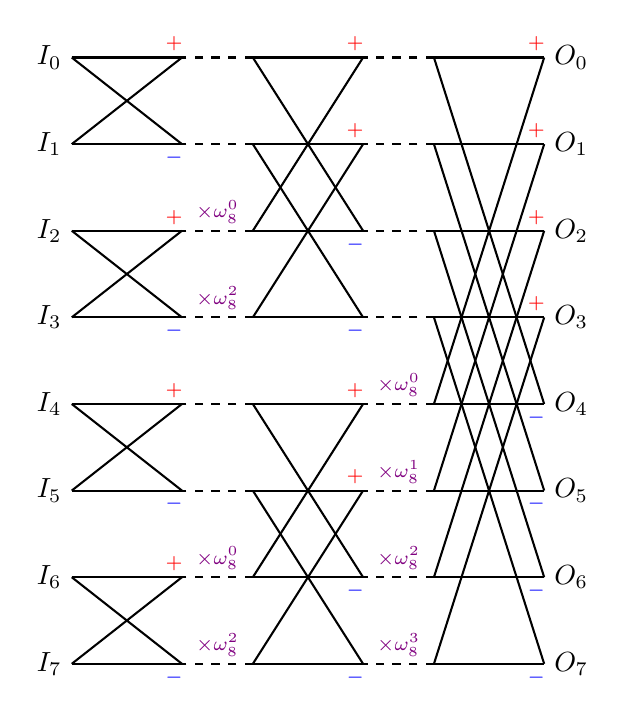
\begin{tikzpicture}[
  % circuit ee IEC,
  >=stealth,
  line width=0.75pt
]%
  \tikzmath{
    \bx = 1.4;      % butterfly width
    \by = -1.1;     % butterfly height
    \sx = 0.9;      % space between stages
    \N  = 8;        % number of points
    \bn = \N/2-1;   % number of butterflies -1
    \sn = ceil{log2(\N)}-1; % number of stages -1 
  }

  \foreach \s in {0,...,\sn} {
    \foreach \b in {0,...,\bn} {
      \tikzmath{
        \gs  = 2^\s;            % group size
        \bg  = mod(\b,\gs);     % butterfly group pos
        \bxp = \sx*\s + \bx*\s; % butterfly x pos
        \byp = 2*\by*\b;        % butterfly y pos
        \w   = int(mod(\b,pow(2,\s)) * pow(2,\sn-\s)); % twiddle factor
        \i1  = int(2*\b);       % input index top
        \i2  = int(2*\b+1);     % input index bot
      }
      % Inputs/Outputs
      \ifthenelse{\s=0}{
        \node[left] at (\bxp cm, \byp cm) {$I_{\i1}$};
        \node[left] at (\bxp cm, \byp cm + \by cm) {$I_{\i2}$};
      }{}
      \ifthenelse{\s=\sn}{
        \node[right] at (\bxp cm + \bx cm, \byp cm) {$O_{\i1}$};
        \node[right] at (\bxp cm + \bx cm, \byp cm + \by cm) {$O_{\i2}$};
      }{}

      % Bfly top and bottom
      \draw  (\bxp cm,          \byp cm)
          -- (\bxp cm + \bx cm, \byp cm) 
             (\bxp cm,          \byp cm + \by cm)
          -- (\bxp cm + \bx cm, \byp cm + \by cm)  ;

      % Bfly diagonals
      \draw  (\bxp cm,          \byp cm - \by*\bg cm)
          -- (\bxp cm + \bx cm, \byp cm - \by*\bg cm + \by*\gs cm)
              node[text=blue, below, xshift=-0.1cm, yshift=0.05cm] {\scriptsize$-$}
             (\bxp cm,          \byp cm - \by*\bg cm + \by*\gs cm)
          -- (\bxp cm + \bx cm, \byp cm - \by*\bg cm)
              node[text=red, above, xshift=-0.1cm, yshift=-0.05cm] {\scriptsize$+$};

      \ifthenelse{\not{\s=0}}{
      % Connection grid
      \draw [dashed]
           (\bxp cm,          \byp cm)
        -- (\bxp cm - \sx cm, \byp cm)
           (\bxp cm,          \byp cm + \by cm)
        -- (\bxp cm - \sx cm, \byp cm + \by cm);

      % Twiddle-factor mult
      \path (\bxp cm         , \byp cm - \by*\bg cm + \by*\gs cm)
        --    node[above, yshift=-1]
                {\textcolor{violet}{\scriptsize{$\times\omega^{\w}_{\N}$}}}
            (\bxp cm - \sx cm, \byp cm - \by*\bg cm + \by*\gs cm);
      }{}
    }
  }
  % \pgfmathparse{equal(mod(\bg,2), 0)}
  % \ifthenelse{\pgfmathresult = 1}{
  % \draw (\bx*\s cm + \bx cm,          \byp cm - \by*\bg cm) to [resistor]
  %       (\bx*\s cm + \bx cm + \sx cm, \byp cm - \by*\bg cm);
\end{tikzpicture}
\end{document}
\end{filecontents*}

\begin{filecontents*}[overwrite]{pipeline.tex}
\documentclass[tikz]{standalone}
\begin{document}
\begin{tikzpicture}[
  circuit ee IEC,
  scale=0.75
]%
  % Input bus
  \draw [very thick]
    (0,0) --
    node[xshift=-0.5cm]{/}
    node[above,xshift=-0.5cm,yshift=1mm]{\footnotesize{$N \times 2 \times 24$}}
    (3,0) coordinate (bin)
    (bin) --++ (90:2.5) --++ (0:1)
    (bin) --++ (90:-2.5) --++ (0:1);

  % MUXes
  \draw 
    (4,1) coordinate (O1)--++
    (90:3)  coordinate (A1)--++
    (-30:1) coordinate (B1)--++
    (-90:2) coordinate (C1)--
    cycle
    (4,-1) coordinate--++ 
    (-90:3) coordinate (A2)--++
    (30:1)  coordinate (B2)--++
    (90:2)  coordinate (C2)--
    cycle
    ($(B1)!0.5!(C1)$)--++(0:1) coordinate (bfly0)
    ($(C2)!0.5!(B2)$)--++(0:1) coordinate (bfly1)
    ($(O1)!0.5!(C1)$)
      node[below,yshift=-5]{\scriptsize{$\log_{2}N$}}--++
      (-90:0.4)
    ($(A2)!0.5!(B2)$)
      node[below,yshift=-5]{\scriptsize{$\log_{2}N$}}--++
      (-90:0.4);
  % \foreach \y/\t in {0.1/1,0.2/2,0.3/3,0.4/4,0.5/5,0.6/6,0.7/7,0.8/8} {
    % \draw ($(C)! \y*1.1 !(O)$)--++(180:1) node[left] {$I_\t$};}

  % Butterfly
  \draw
    (bfly0) --++ (0:4) coordinate (bfly2) 
    (bfly1) --++ (0:4) coordinate (bfly3)
    (bfly0) -- (bfly3)
    (bfly1) -- (bfly2);
  \filldraw
    (bfly0) circle (2pt)
    (bfly1) circle (2pt);
  \draw 
    (bfly2) --++ (0:3) coordinate (bout1)
    (bfly3) --++ (0:3) coordinate (bout2);
  \node[text=red,circle,draw,fill=white] at (bfly2) {\scriptsize$+$};
  \node[text=blue,circle,draw,fill=white] at (bfly3) {\scriptsize$-$};

  % Wmul
  \draw ($(bfly3)!0.5!(bout2)$) --++ (-90:3)
    node[rectangle,draw,fill=white] {\scriptsize{LUT}};
  \node[rectangle,draw,fill=white] at ($(bfly3)!0.5!(bout2)$)
    {\textcolor{violet}{\scriptsize{$\times\omega^{n}_{N}$}}};

  % Registers
  \draw
    (bout1) --++ (0:1) coordinate (recursion1)
    (bout2) --++ (0:1) coordinate (recursion2);
  \node[rectangle,draw,fill=white,minimum height=1cm] at (bout1) {\scriptsize{REG}};
  \node[rectangle,draw,fill=white,minimum height=1cm] at (bout2) {\scriptsize{REG}};
  \path
    (recursion1) --++ (0:1) coordinate (cin1)
    (recursion2) --++ (0:1) coordinate (cin2);
  \node at ($(recursion1)!0.5!(cin1)$) {\dots};
  \node at ($(recursion2)!0.5!(cin2)$) {\dots};

  % FFT delimeter
  \path (bout1) -- coordinate (bout0) (bout2);
  \node[
    rectangle,
    draw=blue,
    dashed,
    minimum width=9cm,
    minimum height=7cm,
    xshift=0cm,
    yshift=-0.2cm]
    at ($(bin)!0.5!(bout0)$) {};
  \node[text=blue,above,yshift=3.3cm] at (bin) {FFT};
  \node[text=blue,above,yshift=3.3cm] at (bout0) {$\times \log_{2}N$};

  % CORDIC 1
  \path
    (bout0) --++ (0:6) coordinate (cordic1)
    (cordic1)
      --++ (180:1.5cm)    coordinate (cordic1yin)
      --++ (90:0.6666cm)  coordinate (cordic1xin)
      --++ (-90:1.3222cm) coordinate (cordic1zin)
    (cordic1)
      --++ (0:1.5cm)      coordinate (cordic1yout)
      --++ (90:0.6666cm)  coordinate (cordic1xout)
      --++ (-90:1.3222cm) coordinate (cordic1zout)
    ($(cin1)!0.5!(cin2)$) --++ (0:1) coordinate (cin0);

  \draw 
    (4,1) coordinate (O1)--++
    (90:3)  coordinate (A1)--++
    (-30:1) coordinate (B1)--++
    (-90:2) coordinate (C1)--
    cycle
    (4,-1) coordinate--++ 
    (-90:3) coordinate (A2)--++
    (30:1)  coordinate (B2)--++
    (90:2)  coordinate (C2)--
    cycle
    ($(B1)!0.5!(C1)$)--++(0:1) coordinate (bfly0)
    ($(C2)!0.5!(B2)$)--++(0:1) coordinate (bfly1)
    ($(O1)!0.5!(C1)$)
      node[below,yshift=-5]{\scriptsize{$\log_{2}N$}}--++
      (-90:0.4)
    ($(A2)!0.5!(B2)$)
      node[below,yshift=-5]{\scriptsize{$\log_{2}N$}}--++
      (-90:0.4);

  \draw
    (cin1) --++ (0:1) --++ (-90:2.5cm-0.6666cm) -- (cordic1xin)
    (cordic1zin) --++ (180:1cm) --++ (-90:0.25cm) node[ground,rotate=-90,xshift=0.1cm]{};

  \node[rectangle,draw,fill=white,minimum width=3cm,minimum height=2cm] at (cordic1) {CORDIC};
    
  \node[left] at (cordic1xin)  {\scriptsize{X}};
  \node[left] at (cordic1yin)  {\scriptsize{Y}};
  \node[left] at (cordic1zin)  {\scriptsize{Z}};
  \node[right] at (cordic1xout) {\scriptsize{X}};
  \node[right] at (cordic1yout) {\scriptsize{Y}};
  \node[right] at (cordic1zout) {\scriptsize{Z}};

\end{tikzpicture}
\end{document}
\end{filecontents*}

\begin{document}
  \input{matrix}
  \input{unit_circle}
  \input{fft}
  \input{pipeline}
  \input{plot}
\end{document}